\documentclass[letterpaper,12pt]{book}
\usepackage[utf8]{inputenc}
\usepackage[spanish]{babel}
\usepackage{hyperref} % Para tener enlaces en la tabla de contenidos
\usepackage[absolute]{textpos} % Para poner una imagen completa en la portada
\usepackage{graphicx} % Para incluir imágenes
\usepackage{yfonts,color} % Lindas primeras letras
\usepackage{bookman} % Usar una fuente más elegante
\usepackage[letterpaper, margin=1in]{geometry}

\addto\captionsspanish{\renewcommand{\contentsname}{Índice}} % Cambiar el título de la tabla de contenidos

\title{El Ingenioso Hidalgo don Quijote de la Mancha - Segunda Parte - Primeros Cinco Capítulos de la Aventura}
\author{Miguel de Cervantes Saavedra}
\date{}

\begin{document}
\pagenumbering{gobble}% Remove page numbers (and reset to 1)
\clearpage
\thispagestyle{empty}
\pagenumbering{roman}
\begin{textblock*}{216mm}(0mm,0mm)
  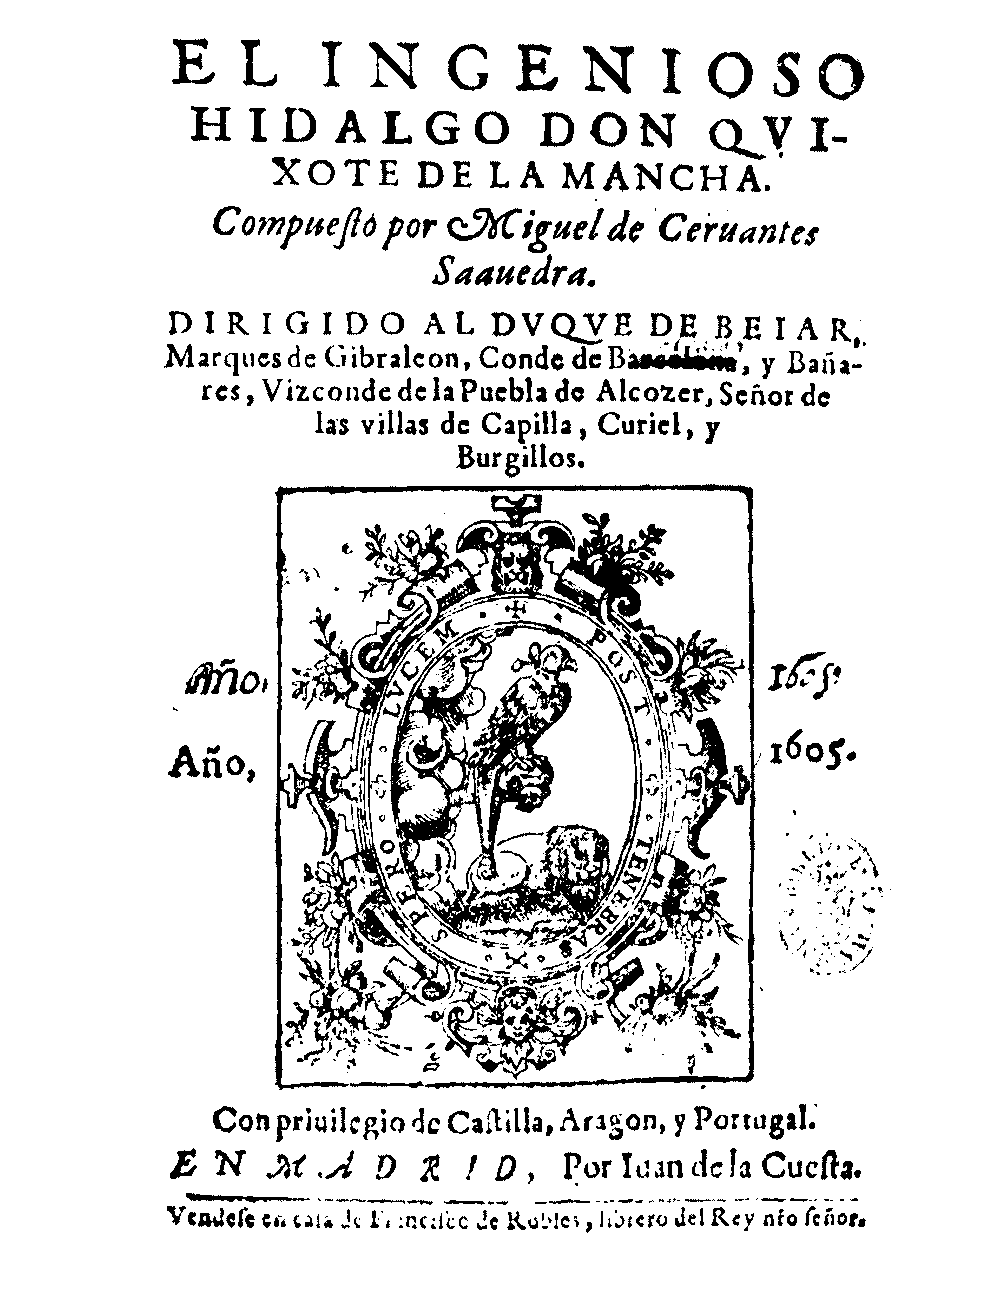
\includegraphics[width=\paperwidth]{cover.png}
\end{textblock*}
	$\,$ % Hack para forzar una primera página sin texto, para que solo tenga la imagen de la portada
	\pagenumbering{gobble}% Remove page numbers (and reset to 1)
\clearpage
\thispagestyle{empty}
\maketitle

\tableofcontents
\addtocontents{toc}{~\hfill\textbf{Pág.}\par}

\chapter[De lo que el cura y el barbero pasaron ...]{De lo que el cura y el barbero pasaron con don Quijote cerca de su enfermedad}
\pagenumbering{arabic}
\input{ch1.txt}

\chapter[Que trata de la notable pendencia ...]{Que trata de la notable pendencia que Sancho Panza tuvo con la sobrina y ama de don Quijote, con otros sujetos graciosos}
\input{ch2.txt}

\chapter[Del ridículo razonamiento ...]{Del ridículo razonamiento que pasó entre don Quijote, Sancho Panza y el bachiller Sansón Carrasco}
\input{ch3.txt}

\chapter[Donde Sancho Panza satisface al ...]{Donde Sancho Panza satisface al bachiller Sansón Carrasco de sus dudas y preguntas, con otros sucesos dignos de saberse y de contarse}
\input{ch4.txt}

\chapter[De la discreta y graciosa plática ...]{De la discreta y graciosa plática que pasó entre Sancho Panza y su mujer Teresa Panza, y otros sucesos dignos de felice recordación }
\input{ch5.txt}

\end{document}